


In \cref{fig:evolution}, we generated similarity plots for the various sites over four eras in order to see how well our groupings based on chemical composition map on to connections posited by historians and archeologists based on a much larger set of data. Because our data comes from a fairly long historical period, we needed to break it up into eras in order to have a well-defined set of historical theories and connections with which to compare it. That is, historians are not generally in the business of theorizing about the connection between Mycenae and Palaiokastro over the entire bronze age, but over much smaller periods. 



\begin{figure}
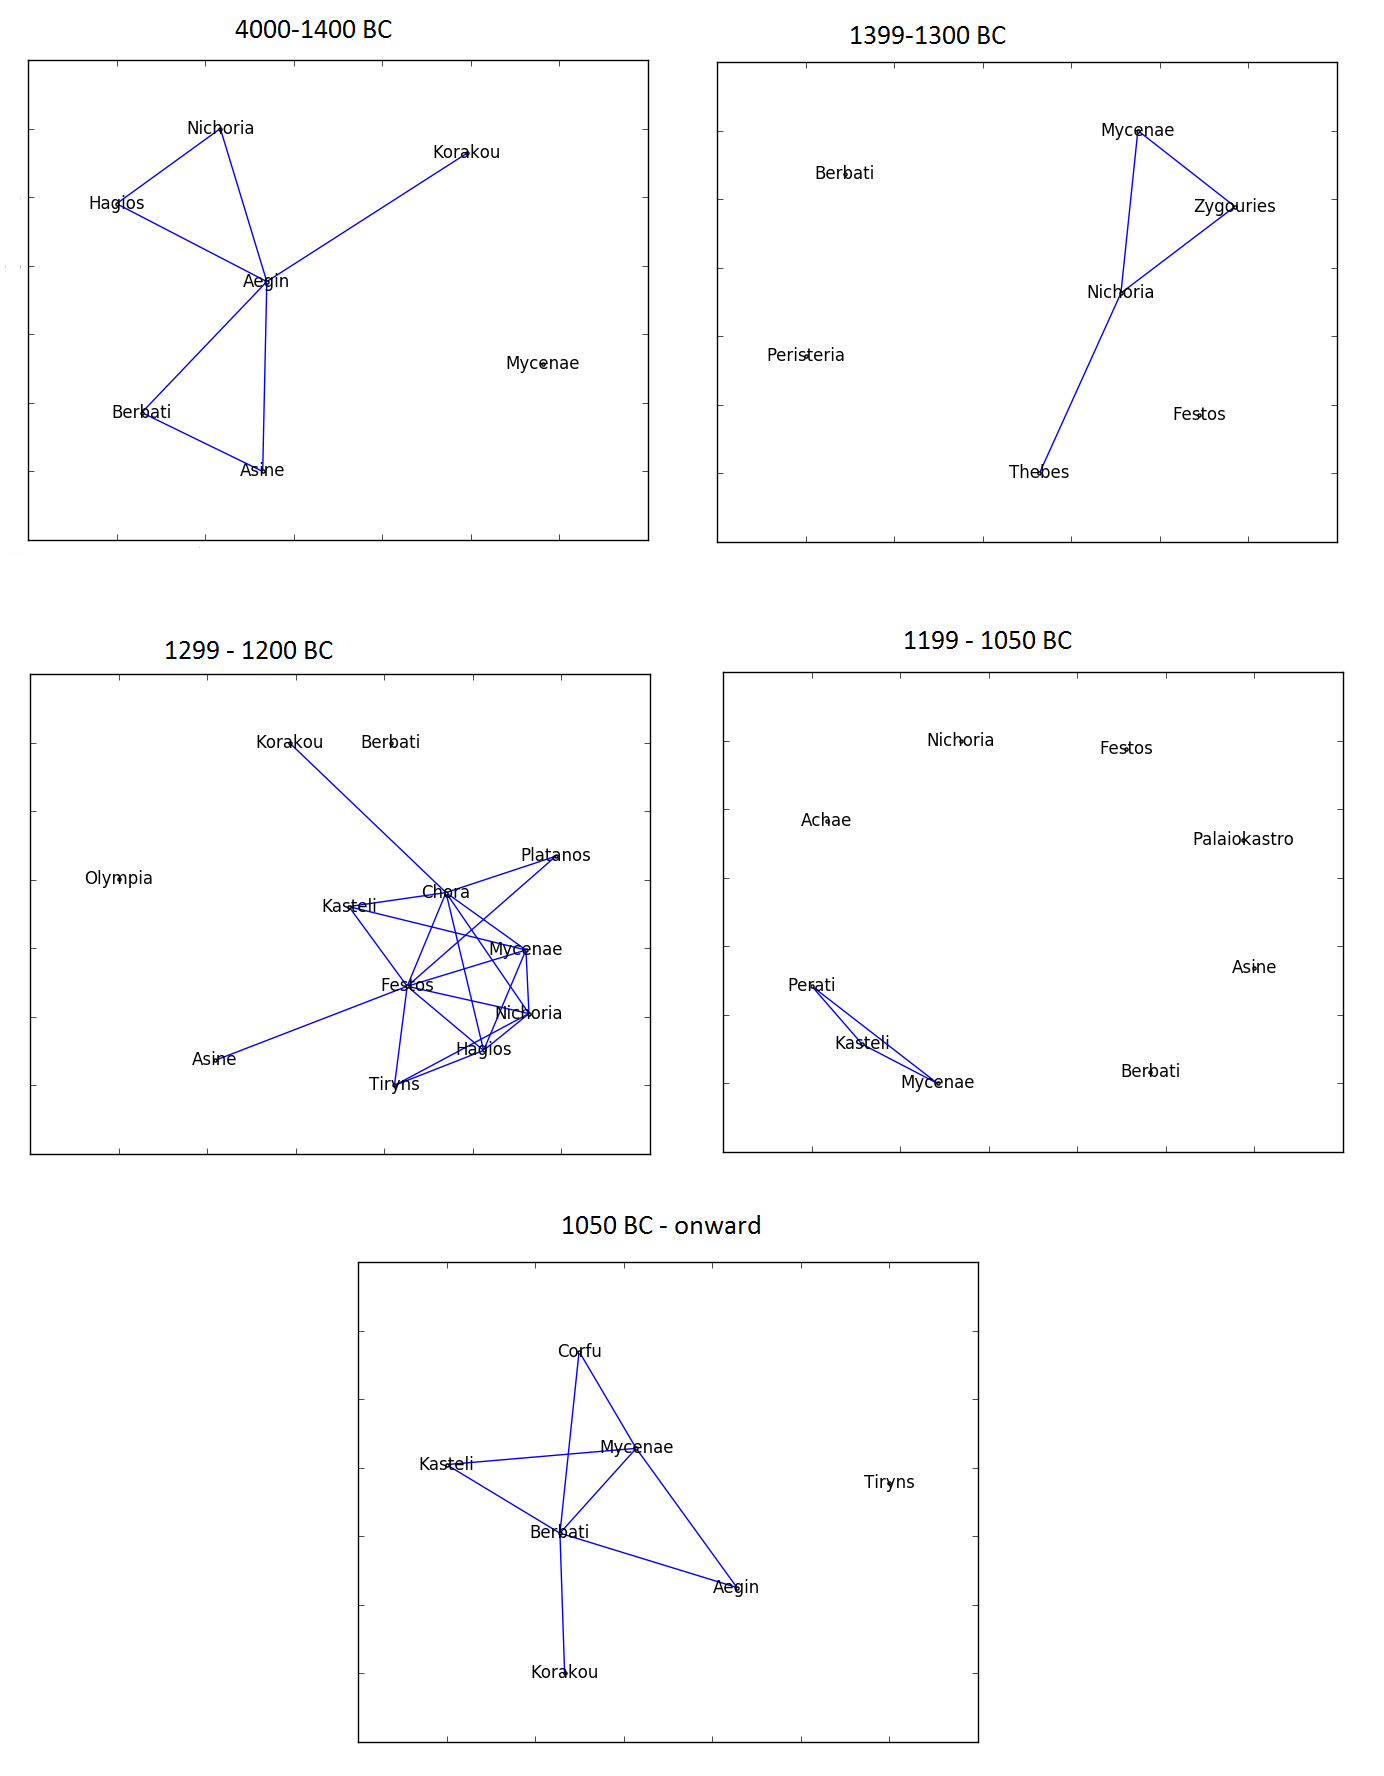
\includegraphics[width=\textwidth]{Network_evolution.png}
\caption{Evolution of networks of the Archaeological sites}
\label{fig:evolution}
\end{figure}


We chose the three later periods based on the standard chronology for bronze age Greece displaying in \cref{fig:timeline}: period 2 (1399-1300) is the Late Helladic III-A, period 3 (1299-1200) is the Late Helladic III-C, and period 4 (1199-1050) is the Late Helladic III-C. The first period includes the earliest artifacts in the dataset; we allowed a much larger period because there were fewer sites and artifacts from this era. 
  
  How many sites in each period?
  
In \cref{fig:evolution}, every site with artifacts dating from that period was included in the graph for that period. The blue links show a kernel-based similarity in the sites based on those artifacts, as described in SECTION. Every similarity measure over a threshold is represented. We chose this threshold based on the histogram of the sum number of connections according to each possible threshold: $10^{5}$ was selected since it was near the median across all eras.

One way of analyzing these plots is to look at the most connected site in each era. A link between sites could represent either geographic factors or cultural-historical ones. Geographic factors include similarity in raw materials available at those sites, either due to proximity or similarity in geographic features such as altitude or distance from bodies of water. Cultural-historical factors include trade, influence and other forms of resettling, conflict and movement of people. For instance, artifacts could reflect trade relations in their chemical composition by actually sharing an origin if they were produced in one site and traded to another, or more indirectly by reflecting similar styles in material, such as a trend in red ware that spread via cultural influence rather than the literal trade in red ware pots. 
 
  
  
For the overall results, the standard historical narrative would predict Mycenae to be fairly central; a vast majority of the artifacts are from the Late Helladic III period, in which Mycenae is the dominant power in the Aegean \cite{demand2011mediterranean}. Our results replicate this: Mycenae is the most connected node in the graph. 



\begin{figure}
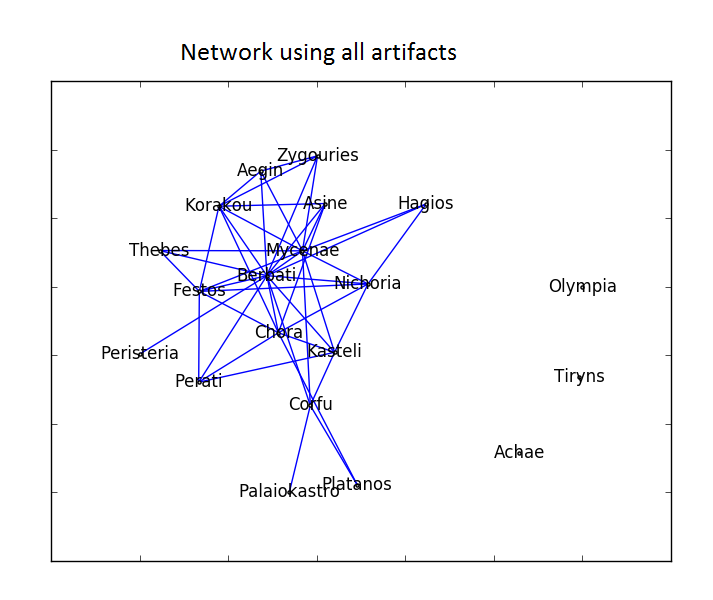
\includegraphics[width=\textwidth]{Overall_Network.png}
\caption{Overall network of the Archaeological sites}
\label{fig:overall}
\end{figure}


\begin{figure}
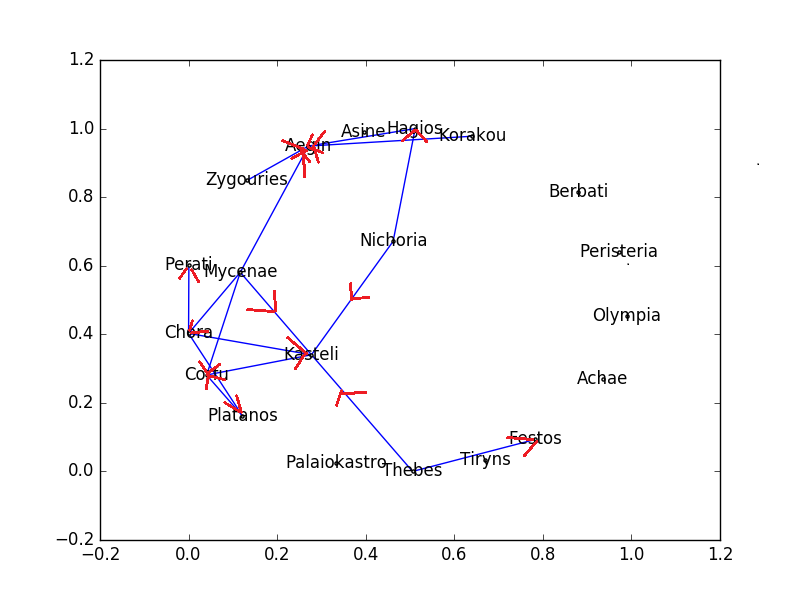
\includegraphics[width=\textwidth]{Overall_network_direct.png}
\caption{Directed network of the Archaeological sites}
\label{fig:overall}
\end{figure}
